\documentclass[runningheads,a4paper,12pt]{report}

\usepackage{geometry}
\usepackage[latin1]{inputenc}
\usepackage{indentfirst} 
\usepackage{multicol}
\usepackage{subcaption}
\usepackage{graphicx}
\usepackage{verbatim} 
\usepackage{gensymb}
\usepackage{amsmath}
\usepackage{float}


\geometry{
 a4paper,
 total={17cm,25.7cm},
 left=2cm,
 top=2cm,
 right=2cm,
 bottom=2cm
 }

\linespread{1.2}

\newtheorem{theorem}{Definition}

\begin{document}

%============== ROMANA ================
\begin{titlepage}
\sloppy
\begin{center}
\Large \textbf{UNIVERSITATEA BABE\c S-BOLYAI, CLUJ NAPOCA}

\Large \textbf{FACULTATEA DE MATEMATIC\u A \c SI INFORMATIC\u A}

\Large \textbf{SPECIALIZAREA INFORMATIC\u A ROM\^ AN\u A}

\vspace{4cm}

\LARGE \textbf{LUCRARE DE LICEN\c T\u A}

\vspace{0.5cm}

\LARGE \textbf {Robo\c ti sociali: detec\c tia emo\c tiilor   prin \^ inv\u a\c tare profund\u a}

\end{center}

\vspace{3cm}

\begin{flushleft}
\LARGE{\textbf{Conduc\u ator \c stiin\c tific}}\\
\LARGE{\textbf{Asist. drd. Miholca Diana-Lucia}}
\end{flushleft}

\vspace{0.3cm}

\begin{flushright}
\LARGE{\textbf{Absolvent}}\\
\LARGE{\textbf{Mardaloescu Ana-Maria}}
\end{flushright}

\vspace{3cm}

\begin{center}
\LARGE{\textbf{2020}}
\end{center}

\newpage

\end{titlepage}


%============== ENGLISH ================
\begin{titlepage}
\sloppy
\begin{center}
\Large \textbf{BABE\c S-BOLYAI UNIVERSITY, CLUJ NAPOCA}

\Large \textbf{FACULTY OF MATHEMATICS AND COMPUTER SCIENCE}

\Large \textbf{SPECIALIZATION COMPUTER SCIENCE}

\vspace{4cm}

\LARGE \textbf{DIPLOMA THESIS}

\vspace{0.3cm}

\LARGE \textbf {Social Robots: Deep Learning based emotion detection}

\end{center}

\vspace{3cm}

\begin{flushleft}
\LARGE{\textbf{Supervisor}}\\
\LARGE{\textbf{Assistant, PhD Student Miholca Diana-Lucia}}
\end{flushleft}

\vspace{0.5cm}

\begin{flushright}
\LARGE{\textbf{Author}}\\
\LARGE{\textbf{Mardaloescu Ana-Maria}}
\end{flushright}

\vspace{3cm}

\begin{center}
\LARGE{\textbf{2020}}
\end{center}

\newpage

\end{titlepage}

\pagenumbering{gobble}

\tableofcontents

\newpage

\pagenumbering{arabic}

\chapter*{Abstract}
\addcontentsline{toc}{chapter}{ABSTRACT} 
The subject of this thesis is the domain of the deep learning in Computer Vision applied in robotics. For this, the Viola-Jones algorithm has been used and integrated in an application to control a robot to recognize its owner, use a convolutional neural network to analyze and predict his or her facial emotion and then to reflect the resulting emotion through a series of suggestive movements. 

The thesis is structured in three chapters. The first chapter presents the theoretical aspects and all the information necessary for understanding this subject. The second chapter focuses on a review of similar projects that have been made and the results that have been achieved. The third chapter is an ample presentation about the proposed application alongside technical details, an user manual and experimental results. Finally, there will be a section of conclusions and future work.  

An original aspect of this thesis consists in presenting, in an original manner, the current state of the art in the field of emotion detection as far as robotics field is concerned. Another original contribution consists in designing, implementing and documenting the application presented in the last chapter for solving the real time emotion recognition algorithm.

This work is the result of my own activity. I have neither given nor received unauthorized assistance on this work. 

\vspace{2cm}

\begin{flushleft}
\textbf{Date: 15.06.2020}
\end{flushleft}

\begin{flushright}
\textbf{Mardaloescu Ana-Maria}\\
\textbf{*semnatura*}
\end{flushright}

\newpage

\addcontentsline{toc}{chapter}{List of Figures} 
\listoffigures

\newpage

\chapter*{Introduction}
\addcontentsline{toc}{chapter}{Introduction} 
Autism Spectrum Disorders (ASD) are a group of life-long disabilities that affect people's communication.
In general, individuals with this kind of disorders have several common features: 1) exhibit strengths in understanding the physical (object-related) world and relative weaknesses in understanding the social world \cite{how-children-with-asd-behave} and 2) are more intrinsically interested in treatment when it involves electronic or robotic components \cite{android-social-skills}.

- autism - improving the social and emotional skills of children with autism

- humans communicate through complex languages (nonverbal cues, such as haptics, kinesics, proxemics and paralanguage)

- For social robots, kinesics is particularly important, as facial expressions play an important role

- the ability to react depending on the emotion of the human lays the foundation for establishing a meaningful nonverbal communication between humans and robots 

- SA FIE INTERESANT SI ATRACTIV, CITITORUL SA VREA SA AFLE MAI MULT

%======== 1.THEORETICAL ASPECTS ========
\chapter{Theoretical aspects}
\label{chapter:theoretical}

This chapter focuses on the theoretical aspects applied in this work and in related experiments. In brief, the presented topics are machine learning, types of learning, types of facial emotion recognition, emotion models and deep learning methods, social robots, as well as a piece of information concerning robotics, electronics and mechanics. 

\section{General}
\label{section:gen}

\subsection{Machine learning}
\label{section:ml}
Ever since computers were invented, people have wondered if they were capable of learning. This fact raised many more questions, the most prominent one being "What does learning mean?" which lead them to start looking for understanding how learning works. Managing to make computers improve themselves based on experience, would be a significant impact. People imagined a whole different world with them mastering machine learning, such as houses learning how to optimize the energy consumption based on their owners' particular usage patterns or computers giving the best treatment for a new disease based on medical records. A truly understanding of the natural process of learning, successfully applied in computer science, would come with new usages of computers and new optimisations of human life, as well as helping people apprehend more about human learning abilities and disabilities. 

A human-like learning computer has not been accomplished yet. However, at the time being it can perform specific tasks and little by little humans discover more and more about the theoretical aspects and stages of the process of learning. 

\begin{figure}
	\centering
	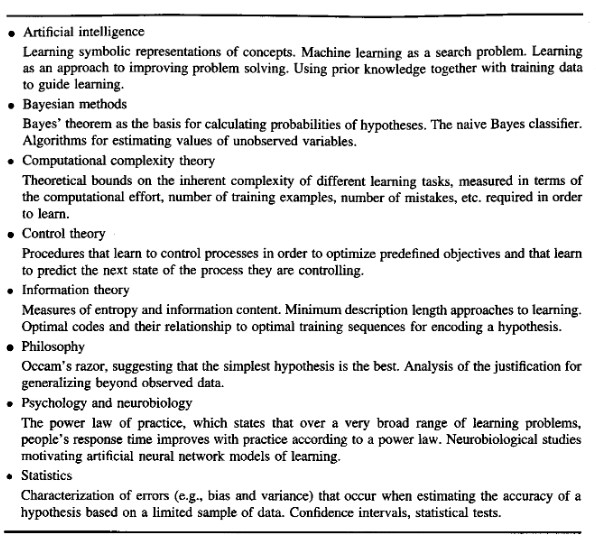
\includegraphics[width=1\linewidth]{./images/1_ml_fields}
	\caption{Fields that had a siginificant impact on machine learning \cite{mitchell}}
	\label{fig:fields}
\end{figure}

Machine learning is a multidisciplinary field. It requires good knowledge of artificial intelligence, probability and statistics, computational complexity theory, control theory, philosophy, psychology, neurobiology and other fields. Figure \ref{fig:fields} summarizes each field's contribution. 

Before going on, the following definition will be introduced, according to \cite{mitchell}:

\begin{theorem}
\label{learning_def}
A computer program is said to learn from experience E with respect to some class of tasks T and performance measure P, if its performance at tasks in T, as measured by P, improves with experience E.
\end{theorem}

To have a well-defined learning problem, there are three features to be identified: the class of tasks, the measure of performance to be improved and the source of experience \cite{mitchell}. The following example is used in order to reinforce the Definition \ref{learning_def} taking into consideration the upper mentioned features: 

\textbf{A computer learning to play Go}
\begin{itemize}
\item Task T: play Go;
\item Source of experience E: practicing against itself or against other opponents;
\item Measure of performance P: percent of games won against opponents. 
\end{itemize}

\subsection{Types of learning}
\label{section:types}
As far as learning problems are concerned, there are three major types of learning: 
\begin{itemize}
\item supervised learning (task driven - predict next value);
\item unsupervised learning (data driven - identify clusters);
\item reinforcement learning (learn from mistakes).
\end{itemize}

\bigskip
\bigskip

\textbf{Supervised learning} uses a model which learns to map between input data and output data, as Bishop stated in his book: 
\emph{"Applications in which the training data comprises examples of the input vectors along with their corresponding target vectors are known as supervised learning problems."} \cite{bishop}. 

Models are trained with a training dataset consisting of input values mapped with output values. The models are adjusted by an algorithm to fit on the training data and predict better. To estimate the performance of the models, they are tested with a testing dataset in which there are given only the input data and the predictions are compared to the output data. 

Supervised learning consists of two main types: 
\begin{itemize}
\item Classification (discrete output) - involves predictiong a class label. An example of a classification problem is plant species classification where the input data are images of different plants and the output data is a class label associated with each image. This type of supervised learning is also called linear regression.
\item Regression (continuous output) - involves predicting a numeric label. An example of regression is average population estimation where the input data are decades starting from the previous century and the output data is an average number of the planet's population associated with each decade. A well-trained model is able to predict the average number of human being for the next decades regarding the last century's growth population. 
\end{itemize}

It is called supervised because the model makes predictions based on its training and during its train it is continuously supervised and revised by an algorithm in order to make better predictions.
\emph{"The term supervised learning originates from the view of the target y being provided by an instructor or teacher who shows the machine learning system what to do."} \cite{deep-learning}

\bigskip
\bigskip

Unlike supervised learning, \textbf{unsupervised learning} does not receive any output data for the training stage and the model has no revision. It uses a model to describe or extract relations between data. 
\emph{"In unsupervised learning, there is no instructor or teacher, and the algorithm must learn to make sense of the data without this guide."} \cite{deep-learning}.

There are two main types of unsupervised learning:
\begin{itemize}
\item clustering - involes finding groups in data. As an example, clustering could be used in analysis of earthquakes: having information about the regions hit by earthquakes, the algorithm can analyse and predict the next probable location of the calamity to occur. 
\item density estimation - involves detection of potential outliers. An application for this algorithm is to view the density of population in different regions of Africa.
\end{itemize}

Both of them can be used for finding patterns in the data. 

\bigskip
\bigskip

The difference between supervised and unsupervised learning is the presence or absence of labeling, but this king of learning is much more distinct from the first two. \textbf{Reinforcement learning} consists of an agent operating in an environment and learning to behave based on a feedback. 
\emph{"Reinforcement learning is learning what to do - how to map situations to actions - so as to maximize a numerical reward signal. The learner is not told which actions to take, but instead must discover which actions yield the most reward by trying them."} \cite{reinforcement-learning-introduction}

At the very beginning, in any environmental conditions, the agent makes a considerable number of mistakes, but as long as it receives a positive signal corresponding to a good behaviour, as well as a negative signal corresponding to a bad behavior, the algorithm is reinforced to prefer good behaviors over the bad ones. The more time it spends running, the less mistakes it learns to make. 

An application in this area is a robot navigating in an environment searching for a target location. It is able to move at any time in one of a number of directions. After several trials it should be able to generate the correct sequence of actions to reach the target location as quickly as possible.  

\subsection{Deep learning methods}
For reaching a higher performance in complex data processing, such as images, recording or videos, a new area of machine learning developed. Deep learning is a specialization of artificial intelligence which uses multiple layers of calculus. 

\subsubsection*{Convolutional Neural Networks}


\subsection{Facial Emotion Recognition methods}
There are three main types of methods as far as facial emotion recognition (FER) is concerned: the holistic methods (modeling the human face deformations globally and encoding them as a whole), the analytical methods (measuring and observing local or distinctive human deformations such as eyes, mouth or nose and their geometrical relationships in order to create expressive models) and hybrid methods (a combination between the two of the above)\cite{automatic-analysis-of-facial-expressions}. 

\subsection{Emotion models}
The way emotions are represented is a basic aspect of a FER system. The Ekman emotion model consists in six basic human emotions: anger, fear, disgust, happy, sadness, surprise \cite{basic-emotions}. OCC (Ortony/Clore/Collins) model is another popular model and it specifies 22 human emotions based on emotional reactions to different situations \cite{the-cognitive-structure-of-emotions}. Plutchik's model defines eight basic bipolar emotions: joy and sadness, anger and fear, trust and disgust, surprise and anticipation \cite{the-nature-of-emotions}.

\section{Social robots}
\label{chapter:social}

\subsection{The general term of "robot"}
Human's creativity manages to find expression in invention as much as in art. Due to the development of technology, robots requests significantly increased. Starting with nature inspired robots, like the ones meant to dangerous or inaccessible environments from Festo\footnote{https://www.festo.com/group/en/cms/10156.htm} or MIT \cite{mit} to nanorobots in the medical field \cite{microrobots}, to hospital assistents or caring robots for the elderly, they come in wider ranges and with more complex functionalities. 

%========= https://learn.g2.com/types-of-robots
There are plenty of factors to take into consideration while classifying robots, but two primary categories differentiate them: movement and use.

As far as locomotion is concerned, robots are classified as:
\begin{multicols}{2}
\begin{itemize}
\item stationary robots;
\item wheeled robots;
\item legged robots;
\item flying robots;
\item swarm robots;
\item nano robots;
\item swimming robots.
\end{itemize}
\end{multicols}

Across the entire field of robotics, a robot's appearance is often informed by the way it moves through an environment, regardless its shape or size. Despite this way of categorizing, many machines that look and move the same may have been designed with distinctive purposes in the real world, which requires consideration from many other angles.

Referring to the various uses of robots, there are six types of them:
\begin{itemize}
\item Industrial robots - the most basic form of machine executing a repetitive task. Due to the fact that they operate in an environment which is free of external influences, they are considered to be the least intelligent form of robot. 
\item Exploration robots - used in dangerous or inaccessible explorations where humans have never gone before. They are used in spatial expeditions, as well as in the deeper corners of the oceans. They are usually equipped with observation and manipulation features, they also have autonomous functions and the capability of being remotely controlled by an operator. 
\item Consumer robots - from cleaning and task-orientated to companionship and sociability. They use artificial intelligence algorithms. 
\item Medical robots - for helping surgeons in delicate operations or for recovery from accidents in the form of exoskeletons. 
\item Aerospace robots - used in research, military intelligence and deep space exploration. They are autonomous or remote controlled drones or spacecraft.
\item Aquatic robots - often used in the biology field to help supplement parts of marine ecosystems that were ravaged by the climate changes.
\end{itemize}

\begin{figure}
	\centering

  \begin{subfigure}{.49\textwidth}
  	\centering
  	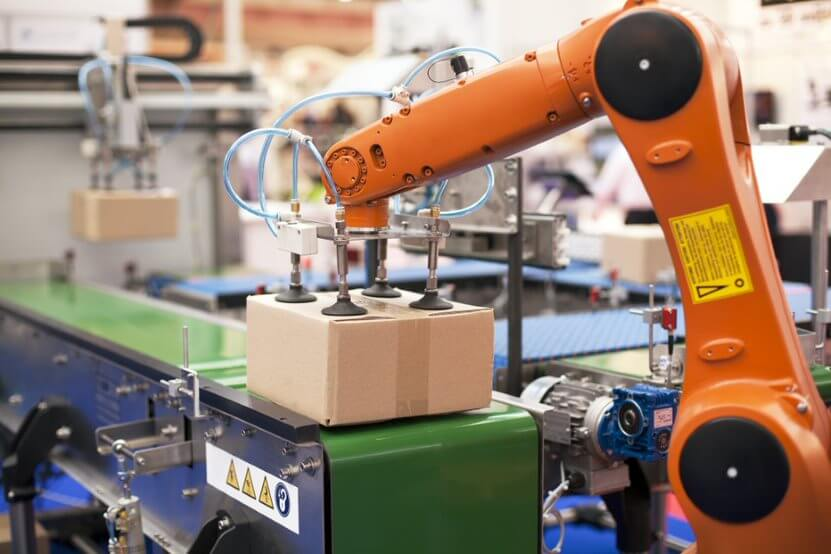
\includegraphics[width=\linewidth]{./images/1_industrial_robot}
  	\caption{}
  	\label{fig:industrial}
  \end{subfigure} 
  %conteaza new line-urile, ai grija 
  \hfill  
  \begin{subfigure}{.46\textwidth}
  	\centering
  	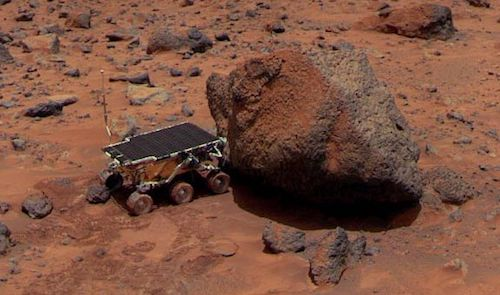
\includegraphics[width=\linewidth]{./images/1_exploration_robot}\hfill
  	\caption{}
  	\label{fig:exploration}
  \end{subfigure}\par\medskip
    
  \begin{subfigure}{.5\textwidth}
  	\centering
  	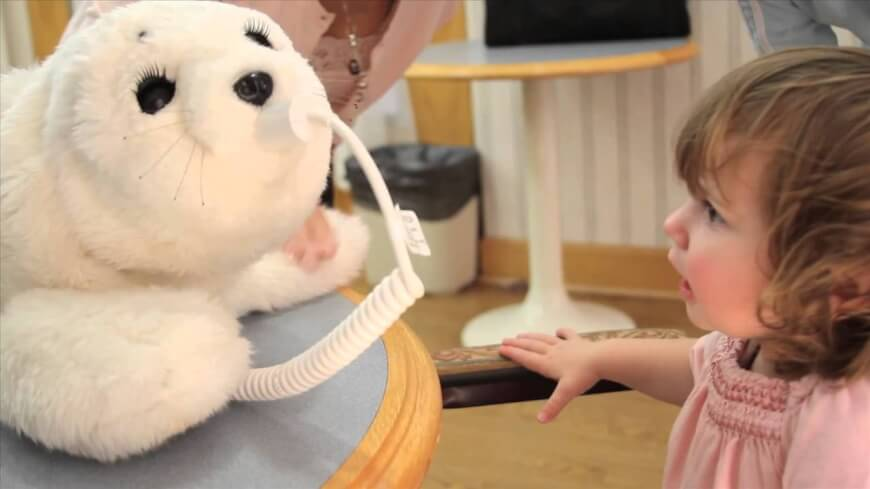
\includegraphics[width=\linewidth]{./images/1_consumer_robot}
  	\caption{}
  	\label{fig:consumer}
  \end{subfigure} 
  \hfill  
  \begin{subfigure}{.45\textwidth}
  	\centering
  	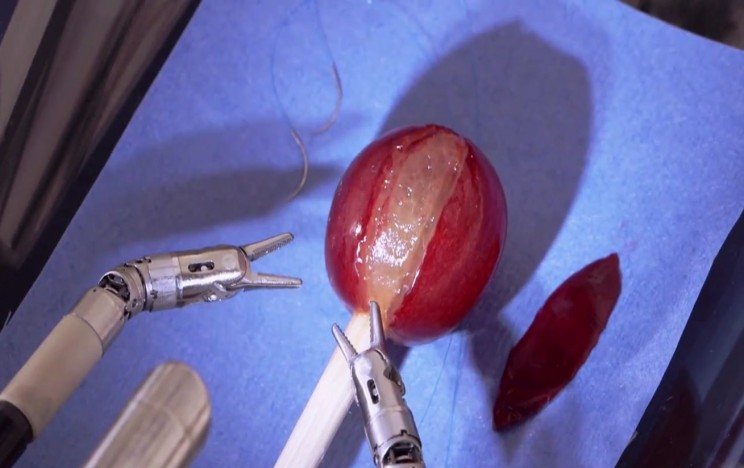
\includegraphics[width=\linewidth]{./images/1_medical_robot}\hfill
  	\caption{}
  	\label{fig:medical}
  \end{subfigure}\par\medskip
  
  \begin{subfigure}{.5\textwidth}
  	\centering
  	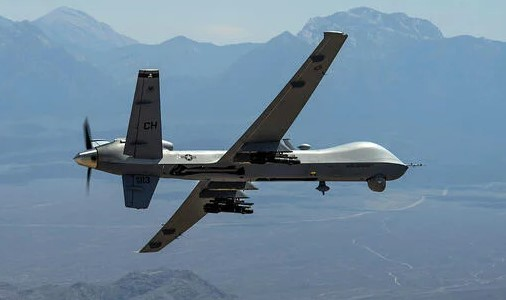
\includegraphics[width=\linewidth]{./images/1_aerospace_robot}
  	\caption{}
  	\label{fig:aerospace}
  \end{subfigure} 
  \hfill  
  \begin{subfigure}{.45\textwidth}
  	\centering
  	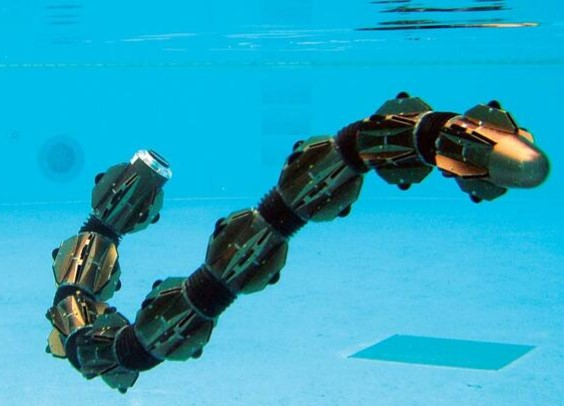
\includegraphics[width=\linewidth]{./images/1_aquatic_robot}\hfill
  	\caption{}
  	\label{fig:aquatic}
  \end{subfigure}\par\medskip  
  
    \caption{Examples of robots. 
    (\subref{fig:industrial}) An industrial robot working in a company. \cite{industrial-robot}
    (\subref{fig:exploration}) A NASA rover as an exploration robot investigating Mars. \cite{exploration-robot}  
    (\subref{fig:consumer}) PARO, an advanced interactive consumer robot, offering animal therapy to patients in a hospital. \cite{consumer-robot}
    (\subref{fig:medical}) A medical robot called daVinci used in tiny incisions with the utmost precision. \cite{medical-robot}
    (\subref{fig:aerospace}) An aerospace robot. \cite{aerospace-robot}
    (\subref{fig:aquatic}) An swimming robot. \cite{aerospace-robot}}
    \label{fig:robot-classification}
\end{figure} 

\subsection{Social robots}
Consumer robots have uses ranging from entertaining audiences to helping people with certain tasks like animal therapy or cleaning a house. A branch of this kind of robots are social robots. 

A social robot is a system based on artificial intelligence which interacts and communicates with people and other autonomous agents. They are designed to interact with people in a natural and interpersonal manner. They have applications in varied fields, such as: education, health, entertainment, communication or research.

Their main and hardest to achieve objective is to become a sufficiently competent partner for humans. They require multiple cognitive abilities, as well as understanding the human brain. This stands in need for a multidisciplinary approach in which the design for a social robot involves wide knowledge of robotics, artificial intelligence, psychology, anthropology and and many more besides. 

Figure \ref{fig:social-robots-fields} illustrates several social robots and their field of work. 

\begin{figure}
	\centering

  \begin{subfigure}{.25\textwidth}
  	\centering
  	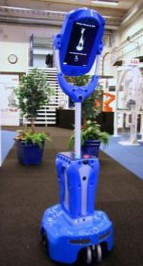
\includegraphics[width=\linewidth]{./images/1_giraff}
  	\caption{}
  	\label{fig:giraff}
  \end{subfigure} 
  %conteaza new line-urile, ai grija 
  \hfill  
  \begin{subfigure}{.3\textwidth}
  	\centering
  	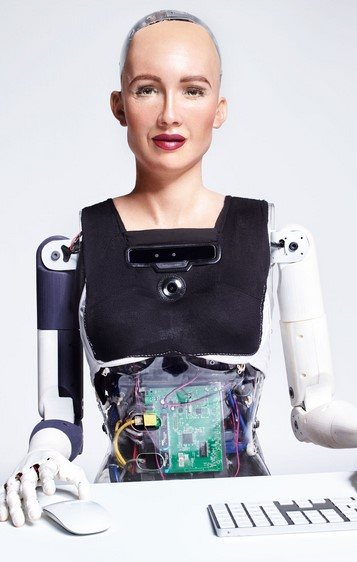
\includegraphics[width=\linewidth]{./images/1_sophia}
  	\caption{}
  	\label{fig:sophia}
  \end{subfigure} 
  \hfill
  \begin{subfigure}{.4\textwidth}
  	\centering
  	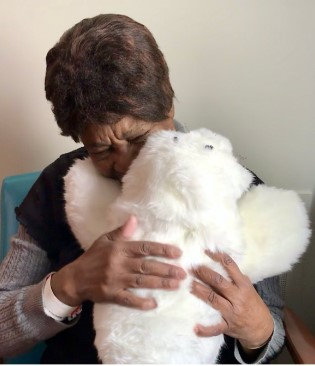
\includegraphics[width=\linewidth]{./images/1_paro}\hfill
  	\caption{}
  	\label{fig:paro}
  \end{subfigure}\par\medskip
  
    \caption{Social robots. 
    (\subref{fig:giraff}) Giraff's purpose is to take care of elderly people. It is composed by a videoconference system enabling communication between pilot users and elderly people. The "head" of the robot has an LCD display showing the avatar of the pilot user. The robotic platform can be controlled through a PC exploiting ad­hoc software. \cite{giraff}
    (\subref{fig:sophia}) Sophia is capable of carrying on an almost normal conversation with a human being. It is also able to draw portraits of people she sees. \cite{sophia}  
    (\subref{fig:paro}) PARO is a social robot used in hostpitals in order to calm down and offer a noral support to elderly people that suffer from cognitive defficiencies. \cite{paro} 
    }
    \label{fig:social-robots-fields}
\end{figure} 

\subsubsection{Medical purposes}

============= to do
Exemple cu Paro, Huggable, etc

\section{Other disciplines related to the concerning thesis}

\subsection{control (firmware)}
\subsubsection{I2C}
\label{section:i2c}
\subsubsection{PWM}
\label{section:pwm}

\subsection{electronics}
\label{section:servomotor}

\subsubsection*{Inverse kinematics}
\label{section:inverse-kinematics}
In mechanical engineering, a kinematic chain is an assembly of rigid bodies connected by joints to provide constrained (or desired) motion that is the mathematical model for a mechanical system. Inverse kinematics is the mathematical process of calculating the variable joint parameters needed to place the end of a kinematic chain.

Given the particular case of a kinematic chain with two segments (figure \ref{fig:1_ik}), the task is to find a solution for q1 and q2 angles with the scope of the end of the kinematic chain, noted with $\xi_E$, to reach a given pair of coordinates (x, y). Each segment has a length, noted with $a_i$, in this case a1 and a2. 

\begin{figure}[h]
	\centering
	\begin{subfigure}{.45\textwidth}
  		\centering
  		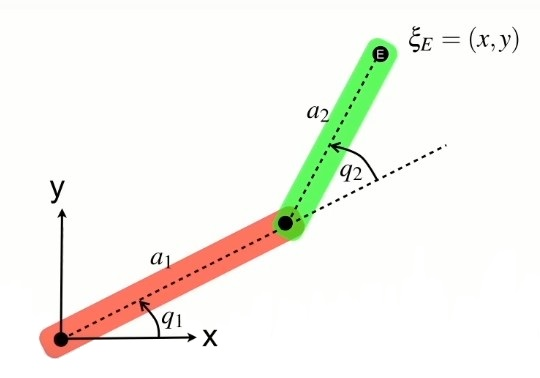
\includegraphics[width=\linewidth]{./images/1_inverse_kinematics}
  		\caption{}
  		\label{fig:ik_a}
  	\end{subfigure} 
  	%conteaza new line-urile, ai grija 
  	\hfill  
  	\begin{subfigure}{.45\textwidth}
  		\centering
  		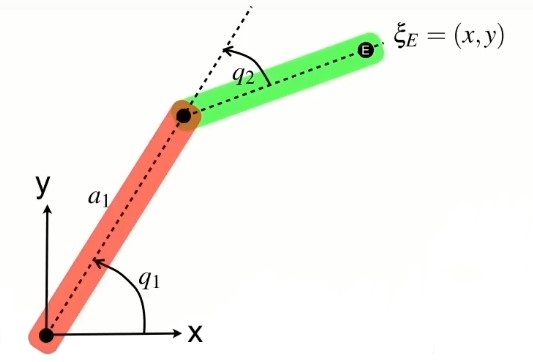
\includegraphics[width=\linewidth]{./images/1_inverse_kinematics2}
  		\caption{}
  		\label{fig:ik_b}
  	\end{subfigure} 
  	\caption{Kinematic chain with two segments}
  	\label{fig:1_ik}
\end{figure}

According to \cite{ik}, following a geometric demonstration, the solution is for 2 cases:

For the case in figure \ref{fig:ik_a}:
\[
    q_2 = \arccos \frac{x^2 + y^2 - a_1^2 - a_2^2}{2 \cdot a_1 \cdot a_2}    
\]
\[
    q_1 = \arctan \frac{y}{x} - \arctan \frac{a_2 \cdot \sin q_2}{a_1 + a2 \cdot \cos q_2}
\]

For the case in figure \ref{fig:ik_b}:
\[
    q_2 = - \arccos \frac{x^2 + y^2 - a_1^2 - a_2^2}{2 \cdot a_1 \cdot a_2}    
\]
\[
    q_1 = \arctan \frac{y}{x} + \arctan \frac{a_2 \cdot \sin q_2}{a_1 + a2 \cdot \cos q_2}
\]

\subsection{mechanics}
despre raspi

despre hat

despre imprimanta 3d

despre servo-uri

schema eletrica?

%======== 2.LITERATURE REVIEW ========
\chapter{Literature review}
\label{chapter:literature}
This chapter focuses on the obtained results of the related approaches in the field of emotion detection applied in robotics using machine learning. These results will serve as a measure reference for my own experimental results. A comparison between different emotion detection algorithms will be made, taking into consideration the hardware constraints and real world practicability. 

\section{Nao humanoid robot}
Nao humanoid robot (HR) is an autonomous, bipedal robot developed by Aldebaran Robotics\footnote{https://www.softbankrobotics.com/emea/en/nao} and it is briefly presented in figure \ref{fig:nao}. In \cite{nao-emotion} there are five stages that lead to the emotion detection: images are taken from Nao's camera, face is detected using Viola-Jones algorithm, facial distances measurements are taken using Geometrik based technique, movements of the measured points are detected using FACS (Facial Action Coding System) and emotion extractions. This paper concentrates only on four emotions: happiness, angriness, sadness and neutral. There was no dataset used in this experiment as emotions where classified based on a labelling system of facial points movements present in the fourth stage. The evaluation results are presented as a confusion matrix in figure \ref{table:nao}.

\begin{figure}[h]
	\centering
  	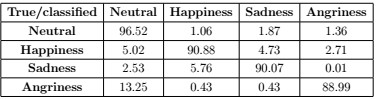
\includegraphics[width=0.7\linewidth]{./images/2_nao_table}
  	\caption{Facial expression rates (\%) \cite{nao-emotion}}
  	\label{table:nao}
\end{figure} 

\begin{figure}[h!]
	\centering
  	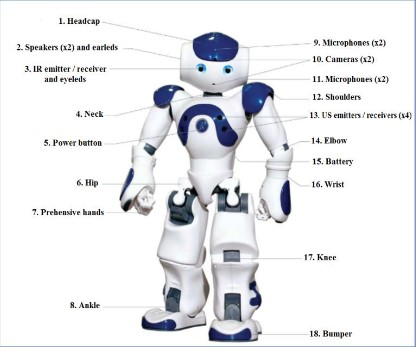
\includegraphics[width=0.6\linewidth]{./images/2_nao}
  	\caption{Nao robot \cite{nao}}
  	\label{fig:nao}
\end{figure} 

In this work, the emotion of anger is the most misclassified - in one out of four cases it is classified as neutral.

\section{Robokind R25 Robot}
R25 social robot has been designed specifically in order to teach children with autism critical social skills. In \cite{automatic-emotion} the facial expression dataset was Cohn-Kanade (CK+) \cite{ck}. There were two conducted experiments: the first one with seven emotions (angry, disgusted, fearful, happy, neutral, sad, surprised) and the second one with six emotions (without "neutral"). The results are presented in figure \ref{fig:ck1}, respectively in figure \ref{fig:ck2}. The happy emotions is the best classified emotion reaching 100\% in all the tests. 

Having an external processing unit, a number of 25 frames processed per second (25fps) was obtained, assuring a natural human-robot interaction.
\begin{figure}
	\centering

  \begin{subfigure}{.45\textwidth}
  	\centering
  	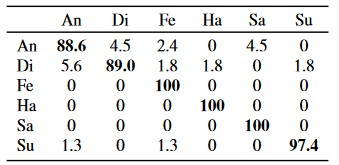
\includegraphics[width=\linewidth]{./images/2_ck1}
  	\caption{}
  	\label{fig:ck1}
  \end{subfigure} 
  %conteaza new line-urile, ai grija 
  \hfill  
  \begin{subfigure}{.45\textwidth}
  	\centering
  	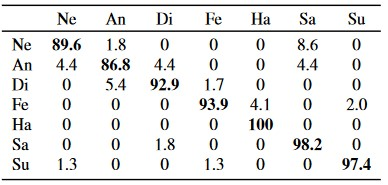
\includegraphics[width=\linewidth]{./images/2_ck2}
  	\caption{}
  	\label{fig:ck2}
  \end{subfigure} 
\end{figure}

==============to continue 

\section{Other papers focused on emotion recognition}

=============== to do

\chapter{The Emotion Cat}
\label{chapter:robot}

The Emotion Cat is the experimental study of this thesis consists of a social robot in the form of a cat which is able to recognize its owner's emotions and adapting its reaction to reflect the read emotion. For that, a holistic method was used for the facial emotion recognition by means of convolutional neural networks. The hardware non-electric parts are an easily assembling puzzle. They were inspired from a robotic cat\footnote{https://cad.onshape.com/documents/a12aa74dd1ae1cffca8aff1a/w/a82fd0f96f82153fa85196a6/e/8908cde

e2b1c43c898434549} and modified or resized as needed. The original design can be found at \cite{nybble}.

\section{Problem definition and functional specifications}
\label{chapter:definition}
The proposed application is a prototype of a social robot which can be used in therapy for people suffering from Autism Spectrum Disorders. The user chooses the owner of the robot to recognize or registers a new owner for the cat. The robot starts scanning and extracting the faces read from the camera and compares them with the images with its owner. If the owner is identified, his face continues being analyzed through a convolutional neural network to predict an emotion which is finally mirrored by the robot in a creative manner. 

The CNN was trained on an Ekman emotion model (with the "neutral" emotion added), called FER-2013 dataset introduced in the ICML 2013 workshop's facial expression recognition challenge \footnote{https://www.kaggle.com/deadskull7/fer2013}. The dataset contains a total of 34034 unique values having a different distribution for each emotion: angry (4953), disgust (547), fear (5121), happy (8989), neutral (6077), sad (4002), surprised (6198). 

The application can be run on a monitor attached to the robot. If no means of displaying are detected, the application starts with a random chosen owner. 

The diagram of the application can be seen at figure X.

=========================== diagrama aplicatiei

\section{Analysis and design}
\label{chapter:analysis}
With its medical as well as entertaining purposes, The Emotion Cat needs an intuitive graphic user interface. Unfortunately, it does not have its own display, thus the robot must be connected to a monitor or TV for the configurations before starting the application. The user is able to choose if he or she wants to keep the monitor connected after starting the application. If the answer is positive, the user will be capable of watching what the robot sees through the camera and how the owner's emotion detection happens.

Considering the storage of the owners' images, there are two possibilities: database or file system. Keeping in mind that the latter one is faster than the read/write operations to a database, the file system is chosen. 

Regardless the mirrored emotions, the robot will not change its spatial coordinates and the user will sit in front of the camera while the application runs. 

\subsection{Graphic user interface}
Tkinter\footnote{https://docs.python.org/3/library/tkinter.html} is the only graphic user interface (GUI) framework which is built in the Python standard library. It is a cross-platform, meaning that it is compatible with either Windows, macOS or Linux with no code changes. Its thin layered object-oriented style makes it easy to use and it is the most common GUI framework used as far as python is concerned. The name comes from "Tk interface" and it was written by Fredrik Lundh.  

Python\footnote{https://www.python.org} is a high-level, object-oriented, interpreted programming language. It has simple and easy to learn syntax, emphasizing readability and, thus, reducing program maintenance. Its implementation started in 1989 by Guido van Rossum. The last version is Python 3.8.

The application has four different windows. The first one is a home window in which the user can choose between the following actions:

\begin{itemize}

\item to register himself/herself as an owner of the robot or to choose his/her name from the already registered names and to start the robot (the second window);

\item (optional) a manual use of the robot (the third window);

\item quitting the application.
\end{itemize}

After starting the application, a new window will show (the fourth window) which will be the camera with the live predictions.

\newpage

\section{Hardware specifications}
Schema eletrica

The Emotion Cat robot used in this thesis is shown in figure \ref{fig:hardware-cat}. The robot is 180mm tall, 215mm long and 100mm wide. It weighs 290 grams. Each leg has 2 servomotors which make possible the move of the robot, one at the hip joint and one at the knee joint, for rotating the upper segment and the lower segment of each leg forward and backward. The micro servos are model SG90 and have a maximum torque 1.8 kg-cm. They may fail to move to the desired position if the torque is insufficient or if the robot weighed more. The current weigh is almost at the edge for the servomotors' torque.

\begin{figure}
	\centering

  \begin{subfigure}{\linewidth}
  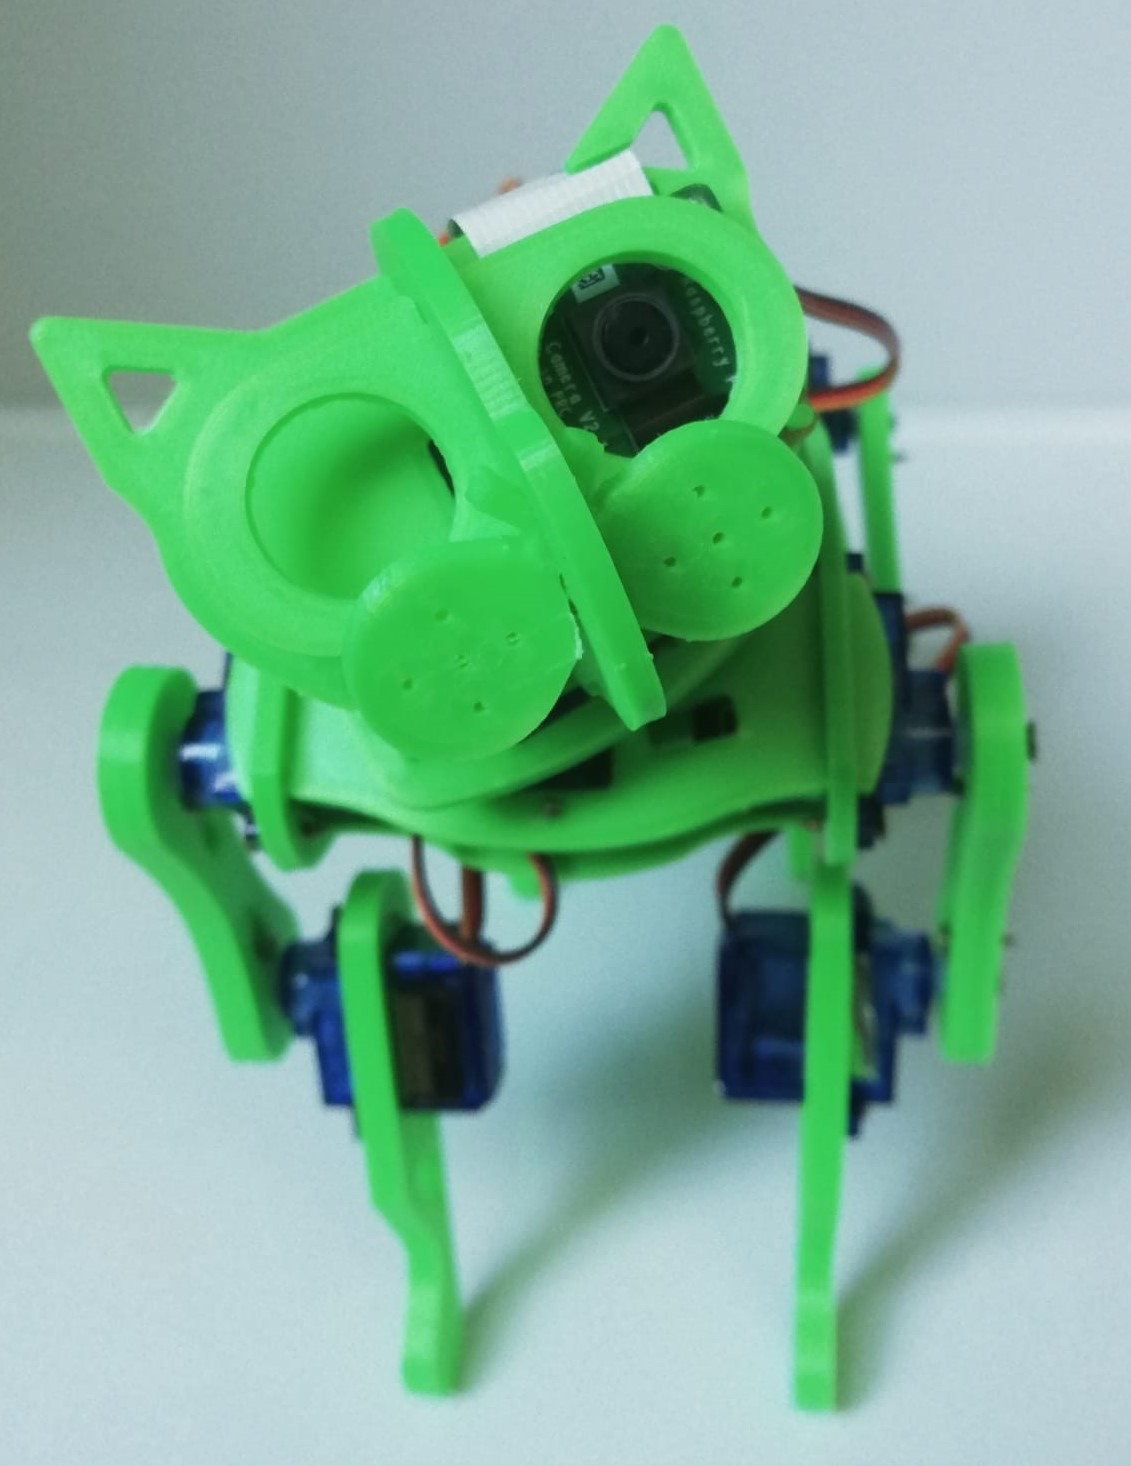
\includegraphics[width=.35\linewidth]{./images/cat_up}\hfill
  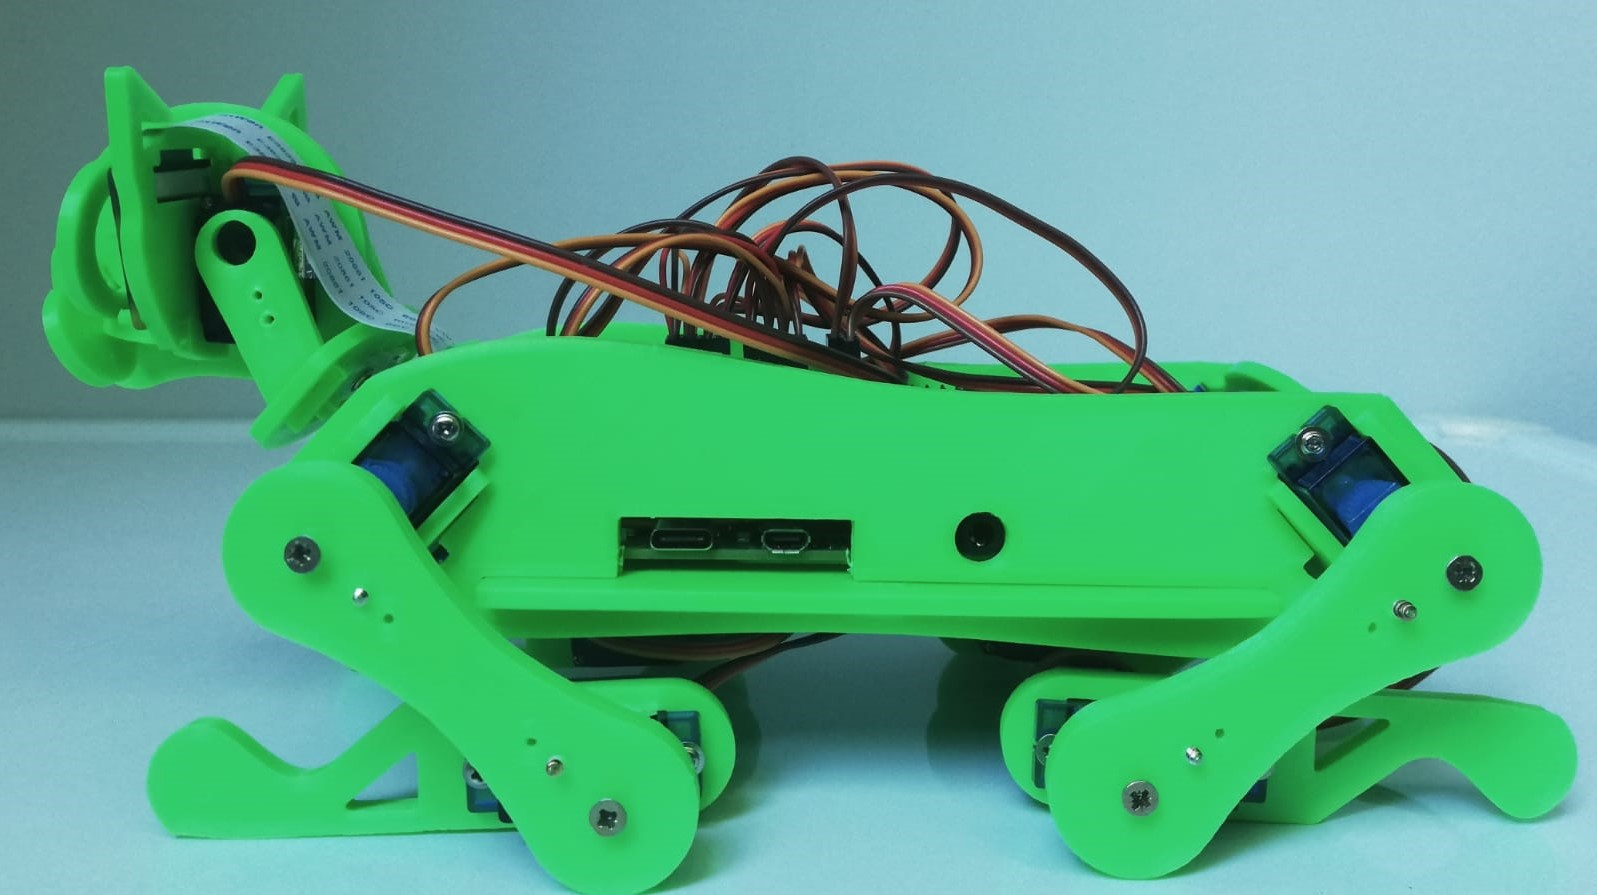
\includegraphics[width=.60\linewidth]{./images/cat_from_lateral}
  \end{subfigure}\par\medskip
  
  \begin{subfigure}{\linewidth}
  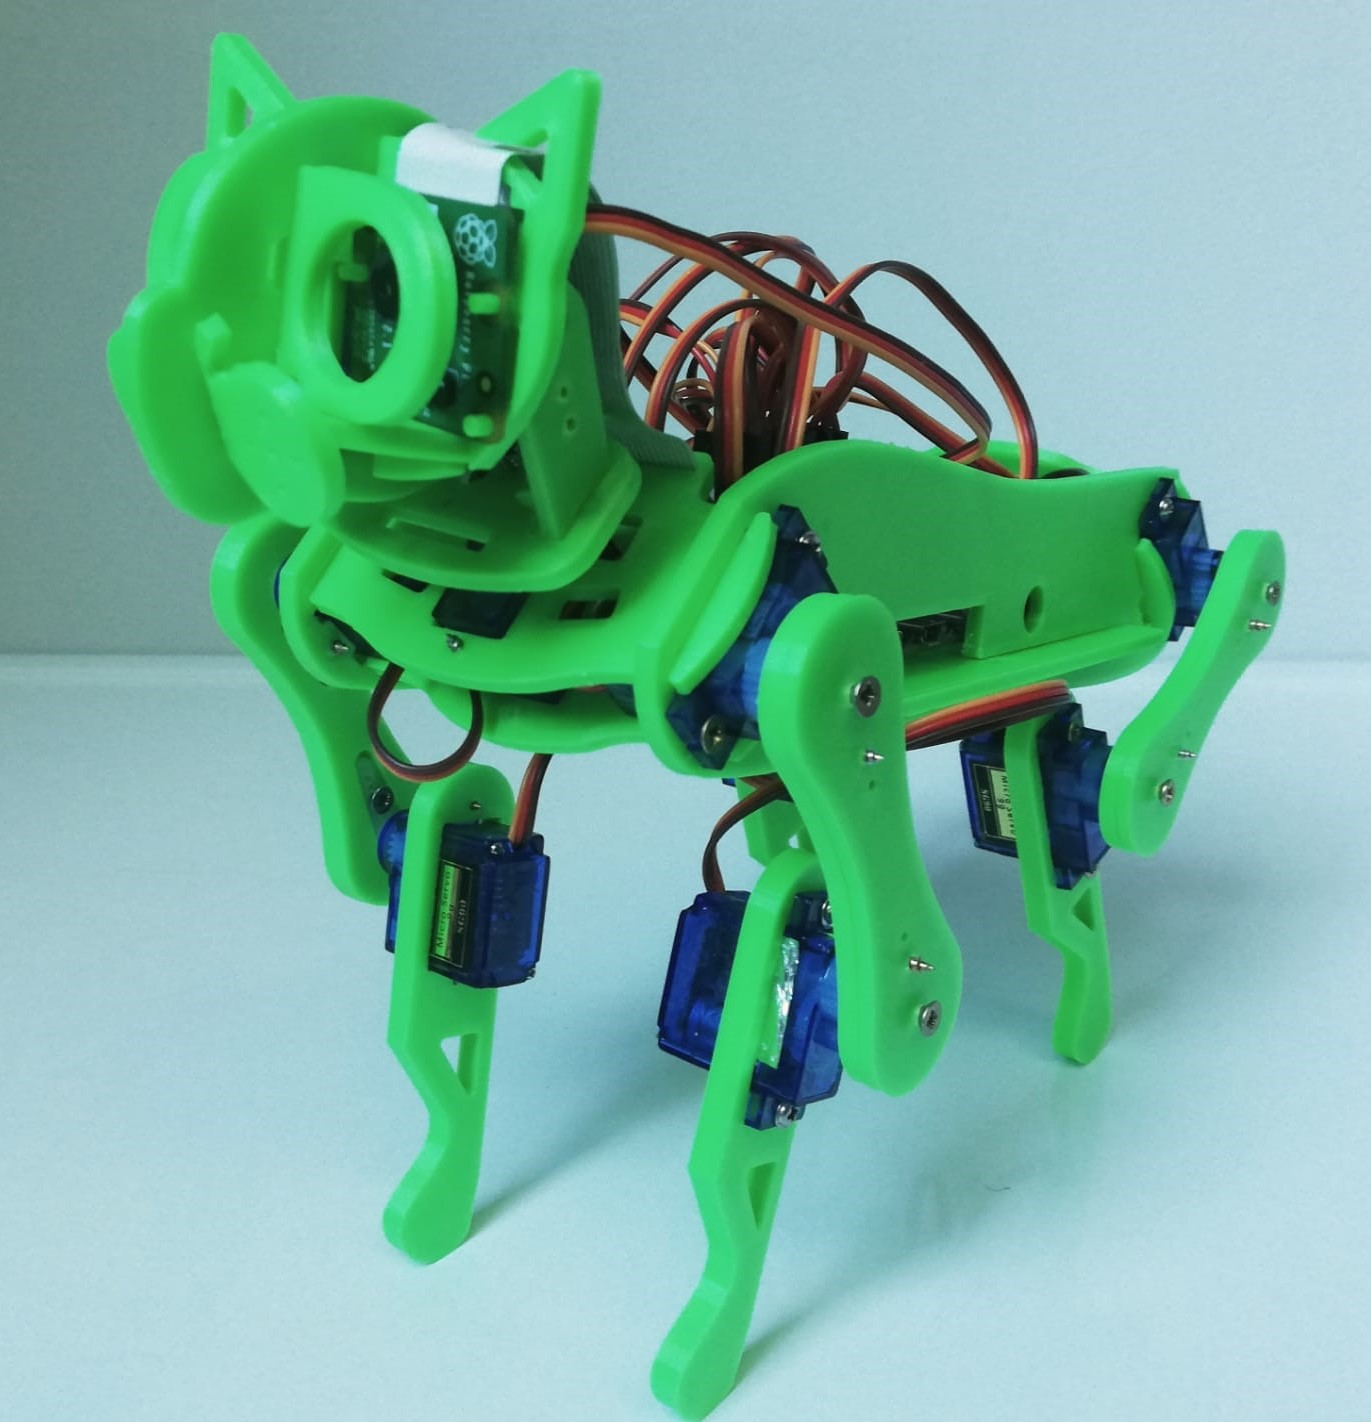
\includegraphics[width=.35\linewidth]{./images/cat_up_izometric}\hfill
  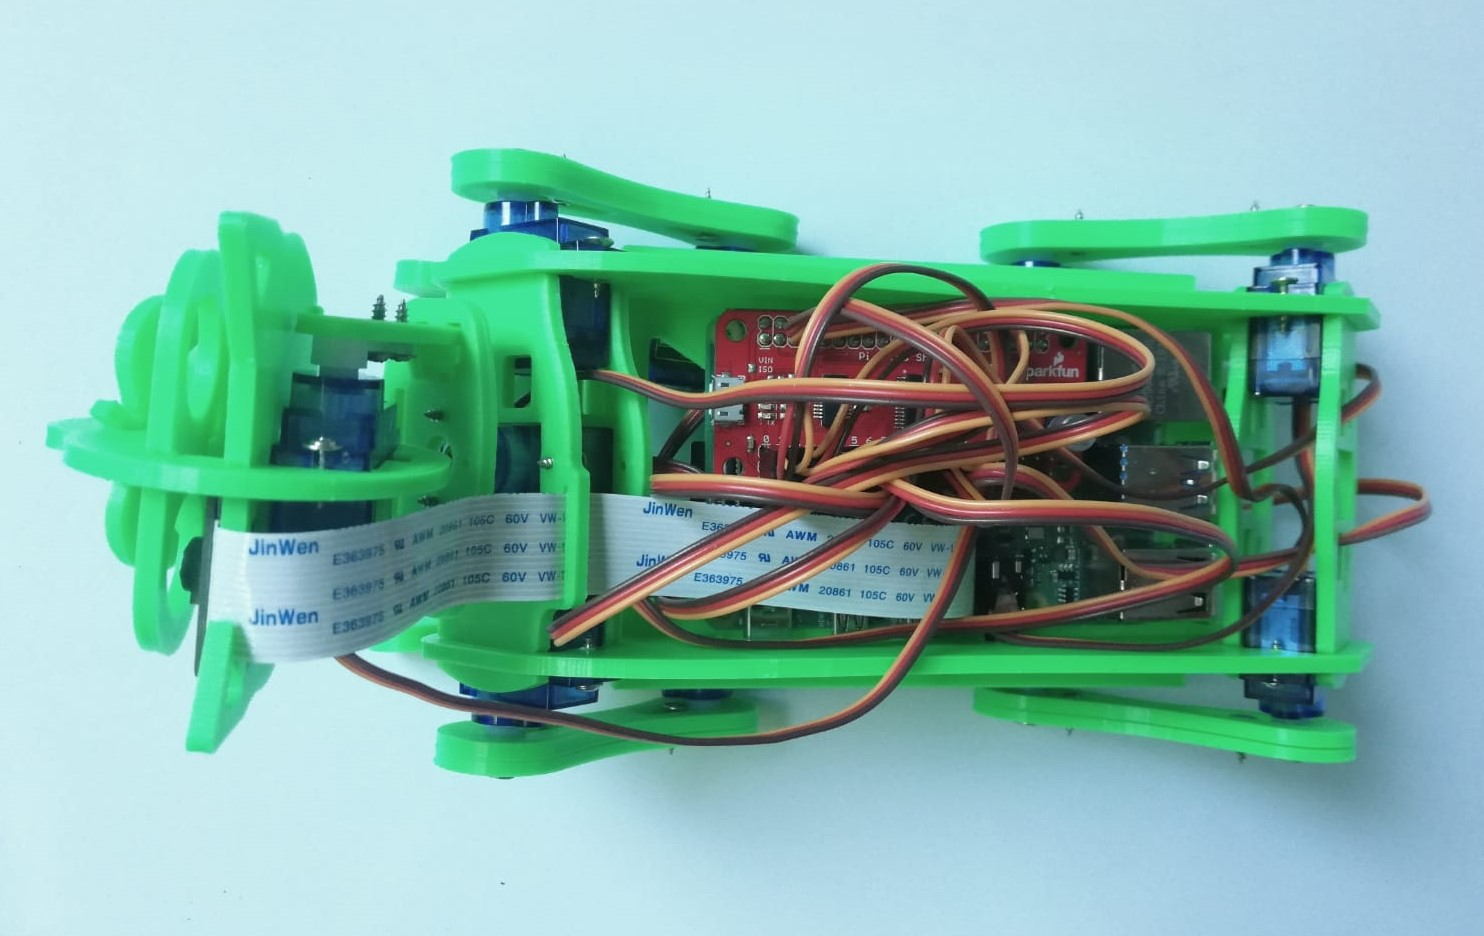
\includegraphics[width=.60\linewidth]{./images/cat_from_above}
  \end{subfigure}
    
    \caption{The Emotion Cat}  
    \label{fig:hardware-cat}
\end{figure} 

\subsection*{Raspberry Pi}
The most important part of the hardware section is the Raspberry Pi 4 Computer\footnote{https://www.raspberrypi.org}, Model B, consisting of 2 GB of RAM (figure \ref{fig:raspi}). It has the following specifications:
\begin{multicols}{2}
\begin{itemize}
\item 64-bit quad-core Cortex-A72 processor;
\item 2GB LPDDR4 RAM;
\item 2 micro HDMI ports (supports up to 4Kp60);
\item 2 USB 3.0 ports;
\item 2 USB 2.0 ports;
\item Gigabit Ethernet port
\item 802.11b/g/n/ac wireless;
\item Bluetooth 5.0;
\item PoE-capable (requires PoE HAT, sold separately);
\item 5V/3A USB-C power supply required (sold separately)
\end{itemize}
\end{multicols}

This board runs Raspberry Pi OS which is a version of Linux. This is the computer that runs the proposed application. 

\begin{figure}
	\centering
	
	\begin{subfigure}{\linewidth}
  		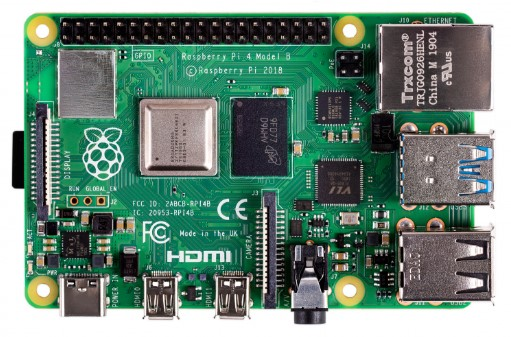
\includegraphics[width=.45\linewidth]{./images/3_raspberrypi1}\hfill
  		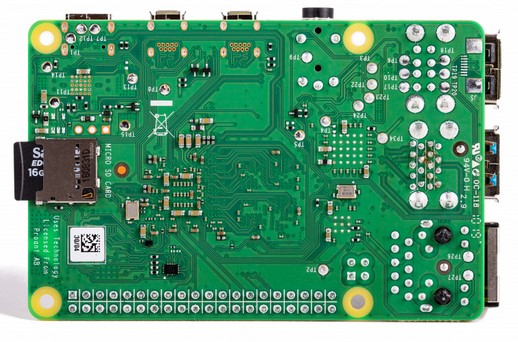
\includegraphics[width=.45\linewidth]{./images/3_raspberrypi2}
  	\end{subfigure}
    
    \caption{Raspberry Pi 4}  
    \label{fig:raspi}
\end{figure}

\subsection*{Pi Camera}
The Camera Module V2\footnote{https://www.raspberrypi.org/products/camera-module-v2/} is compatible with all version of the Raspberry Pi board. It replaced the original Camera Module in April 2016. This version has a Sony IMX219 8-megapixel sensor, so it can be used in high-definition videos, as well as photographs. 

In this project, only one Pi Camera is used as the left eye of the robot, which can be seen in figure \ref{fig:hardware-cat}.

\subsection*{SparkFun Pi Hat}
The SparkFun Pi Hat\footnote{https://learn.sparkfun.com/tutorials/pi-servo-hat-hookup-guide/all} is a servo driver which is attached to the Rasbperry Pi. It is able to control up to 16 servo motors via $I^2C$ connection. It can also be powered separately from the board.

The first channel has the starting address at 0x06 and the stop address at 0x08. Simply increasing the address of the two registers above by 4, the following channel's registers will result. Thus, the start address for channel 1 is 0x0A and the stop address is 0x0C, for channel 2 0x0E and 0x10 and so on. The complete list of addreses for each channel is in figure \ref{fig:hat-addresses}.

\begin{figure}
	\centering

  	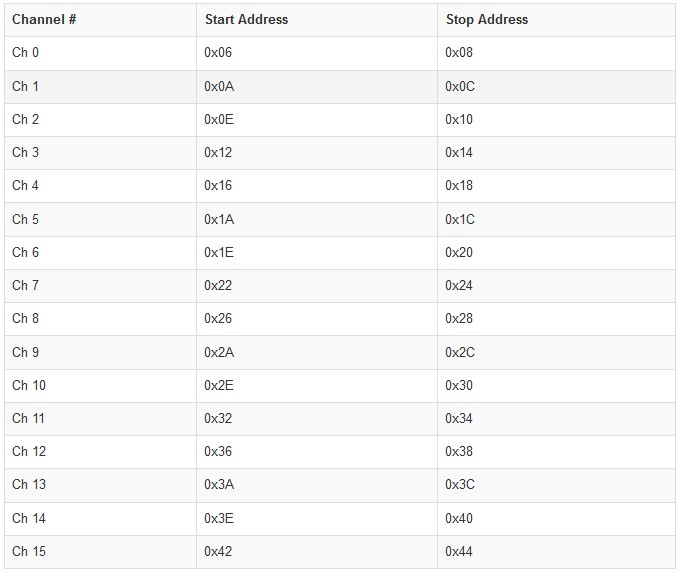
\includegraphics[width=\linewidth]{./images/3_hat_addresses}\hfill

    \caption{SparkFun Pi Hat: the start and stop address corresponding to each channel.}  
    \label{fig:hat-addresses}
\end{figure}

\begin{figure}
	\centering

  	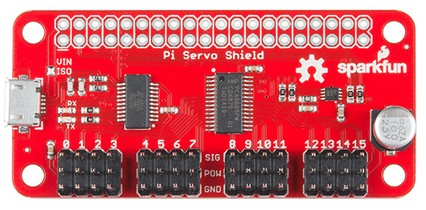
\includegraphics[width=.6\linewidth]{./images/3_hat}\hfill

    \caption{SparkFun Pi Hat}  
    \label{fig:hat}
\end{figure}

\subsection*{Servomotors}
The Emotion Cat consists of 11 Micro Servomotors SG90 90\textdegree\footnote{https://datasheetspdf.com/pdf/791970/TowerPro/SG90/1}: 2 for each leg, 2 for head and 1 for tail. Even though they are for hobbyists, they have high output power and a decent accuracy. They can be seen in figure \ref{fig:servo}.

\begin{figure}
	\centering

  	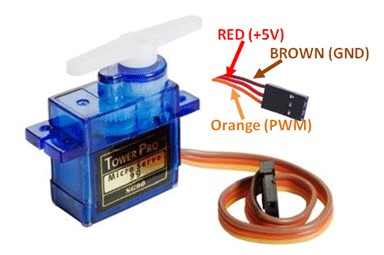
\includegraphics[width=.6\linewidth]{./images/3_servo}\hfill

    \caption{Micro Servomotor SG90 90\textdegree}  
    \label{fig:servo}
\end{figure}

\subsection*{3D printed parts}
The rest of the robot is 3D printed and consists of 15 different pieces and 30 in total with a thickness of 3 millimeters each. They were mechanically designed using the computer program SolidWorks\footnote{https://www.solidworks.com/}, prepared for printing via a slicing application for 3D printers, called Cura\footnote{https://ultimaker.com/software/ultimaker-cura} and, finally, 3D printed\footnote{https://www.creality3dofficial.com/products/creality-ender-3-pro-3d-printer}.  

\subsection*{Assemble}
The mechanical design and assemble can be seen in figure \ref{fig:3_hardware}, as well as figure \ref{fig:3_hardware2} with different views. Several changes were made in order to adapt the robot to the current tasks: in figure \ref{fig:3_lateral} there are 2 orifices for power supplying and monitor connecting purposes, the holes in the support of the Raspberry Pi board in figure \ref{fig:3_bottom} as a cooling method, 3 little mechanical pins for the camera fixation in figure \ref{fig:3_front}. The tail helps the robot to balance.
==============spune despre papucii din cauciuc

\begin{figure}
	\centering

  	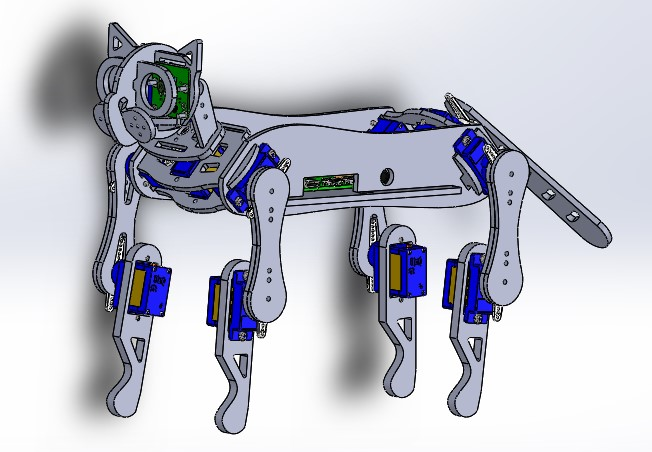
\includegraphics[width=.6\linewidth]{./images/3_hardware}\hfill

    \caption{Isometric view of the assemble in SolidWorks}  
    \label{fig:3_hardware}
\end{figure}


\begin{figure}[H]
	\centering
	\begin{subfigure}{.3\textwidth}
  		\centering
  		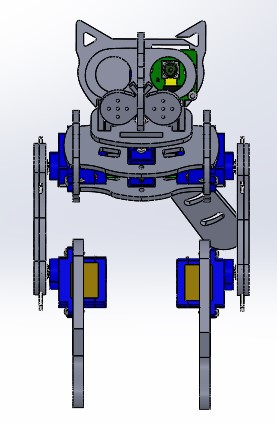
\includegraphics[width=\linewidth]{./images/3_hard_face}
  		\caption{}
  		\label{fig:3_frontal}
  	\end{subfigure} 
  	%conteaza new line-urile, ai grija 
  	\hfill  
  	\begin{subfigure}{.2\textwidth}
  		\centering
  		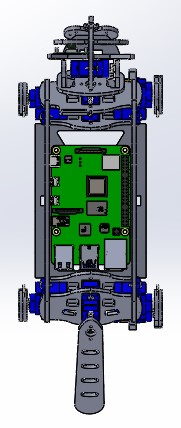
\includegraphics[width=\linewidth]{./images/3_hard_up}
  		\caption{}
  		\label{fig:3_top}
  	\end{subfigure}
  	\hfill  
  	\begin{subfigure}{.25\textwidth}
  		\centering
  		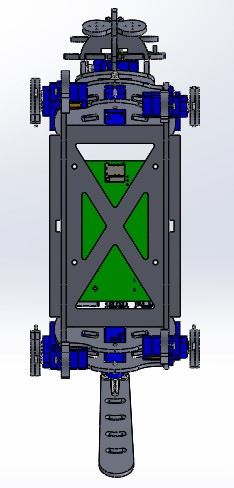
\includegraphics[width=\linewidth]{./images/3_hard_down}
  		\caption{}
  		\label{fig:3_bottom}
  	\end{subfigure}
  	
  	\begin{subfigure}{0.5\textwidth}
  		\centering
  		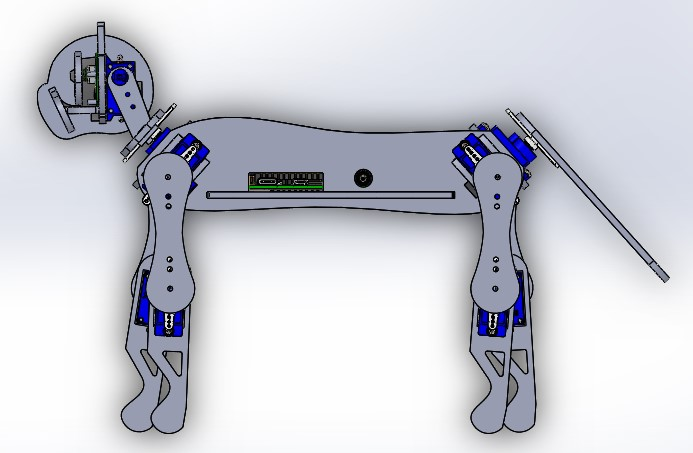
\includegraphics[width=\linewidth]{./images/3_hard_lateral}
  		\caption{}
  		\label{fig:3_lateral}
  	\end{subfigure}
  	\caption{Robot assemble: 
  		(\subref{fig:3_frontal}) frontal view,
  		(\subref{fig:3_top}) top view,
  		(\subref{fig:3_bottom}) bottom view,
  		(\subref{fig:3_lateral}) lateral view.
  		}
  	\label{fig:3_hardware2}
\end{figure}

\newpage

\section{Implementation}
\label{chapter:implementation}

Modular programming refers to the process of breaking a large and complex task into separate, simpler subtasks. Modularizing code in a large application has several advantages: simplicity (each module focuses on a part of the problem), maintainability (enforcing logical boundaries between different problem domains), reusability (reducing duplicate code by reusing an already defined functionality in a module) and scoping (avoiding collisions). 

The proposed method uses a two-level hierarchical decomposition of the task. Given the started application with a chosen owner and the working camera with a face in the frame, the high-level part has to compare and recognize the face and predict the recognized owner's emotion. It is then the low-level's controller's task to move the robot's body (feet, head and tail) in order to reflect the predicted emotion. 

For keeping the dependencies required by this application isolated, the Python 3 virtual environment tools virtualenv\footnote{https://virtualenv.pypa.io/en/latest/} and virtualenvwrapper\footnote{https://virtualenvwrapper.readthedocs.io/en/latest/} were used. 

\subsection*{Low-level controller}
The job of the low-level controller is to output servomotors commands that will move the entire body in a position reflecting an emotion.

It is divided into four packages: domain, persistence, services and validation. 

\subsubsection{Domain}
The domain handles the communication between software and hardware using an $I^2C$ (see \ref{section:i2c}) bus reffered to as SMBus. The entities Leg, Tail and Head implement the ILimb interface which confers them the move method with a list of parameters differing from the limb class:
\begin{itemize}
\item Leg - requests a list of two parameters standing for the two coordinates in the XOY system in which the leg is positioned;
\item Tail - requests a list of two parameters standing for the servomotor angle and the speed of movement;
\item Head - requests a list of three parameters standing for the upper servomotor angle, the lower servomotor angle and the speed of movement.
\end{itemize}

With two servomotors to control, both Leg and Head classes invoke one thread per servomotor in order to parallelize the commands. For a closer look to reality, the transition from the current angle to the new one should be as smooth as possible, so the servomotor goes through a set of intermediate states that brings it closer to the next angle with a given step size. The greater the step size, the fewer the intermediate states  and the faster it will reach the goal angle. 

The leg angles calculations are obtained using inverse kinematics (see \ref{section:inverse-kinematics}), applying the formulas for the case showed in figure \ref{fig:ik_a} with the difference that the starting position of the kinematic chain has the 2 segments at an angle of 50\textdegree. The resulted angles are corrected according to the specific leg, after the following rule:

\begin{equation*}
    corrected\_angle = \begin{cases}
               current\_angle  & \text{if leg is on the right side,}\\
               90 - current\_angle  & \text{otherwise.}\\
               \end{cases}
\end{equation*}

In other words, the left side legs mirror the right side legs, so they require a complementary angle. This is due to the inverse kinematics formulas that were made considering the right side legs. 

The process of moving a servomotor needs two signal commands. The first write is to the "start time" register. By default, the PWM (see \ref{section:pwm}) frequency of the chip is 200Hz, or one pulse every 5ms. The start time register determines when the pulse goes high in the 5ms cycle. All channels are synchronized to that cycle. Generally, this should be written to 0. The second write is to the "stop time" register, and it controls when the pulse should go low. The range for this value is from 0 to 4095 (in this application, the three main reference values are: 836 for 0\textdegree, 1250 for 45\textdegree, 1664 for 90\textdegree), and each count represents one slice of that 5ms period (5ms/4095), or about 1.2$\mu$s ($1.2 \cdot 10^{-6}$ seconds). Thus, the value of 1250 written above represents about 1.5ms of high time per 5ms period. Servo motors get their control signal from that pulse width. Here, the formula to calculate the pulse from degrees is: 

\[pulse\_var = 836 + 9.2 * degree\_var\]

\subsubsection{Validation}
This package's job is data validations. Before an angle is sent as a signal to the servomotor, it is validated to belong to the domain of definition (in this case (0\textdegree; 90\textdegree)). In case of an out of the domain of definition angle, the robot will not execute the given commands and will wait for the next valid set of commands.

\subsubsection{Persistence}
The persistence package handles the file reading and offers all the information about the addresses of the Pi Hat's channels in order to control the servomotors. 

\subsubsection{Services}
The services package handles the logic and the control of the low-level section of he application. It contains three classes: ControllerLimb, Mover and DecisionMaker. For logic comprehension, the explanation will be in the top-down style as following: 

\begin{figure}
	\centering

  	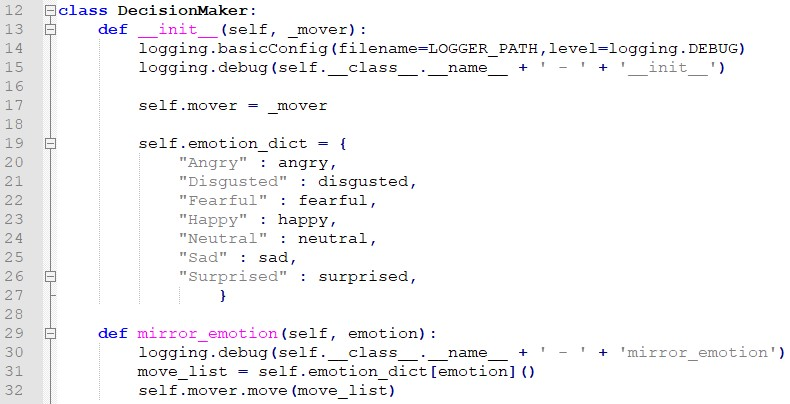
\includegraphics[width=\linewidth]{./images/3_decision_maker}\hfill

    \caption{DecisionMaker class}  
    \label{fig:decision-maker}
\end{figure}

DecisionMaker (figure \ref{fig:decision-maker}) receives one emotion through the method mirror\_emotion and decides which set of movements the robot should do according to the given emotion. It has an emotion dictionary (line 19) with a string signifying an emotion as a key and  a function as a value. The seven functions return a list of movements that is handled by a Mover object. 

\begin{figure}
	\centering

  	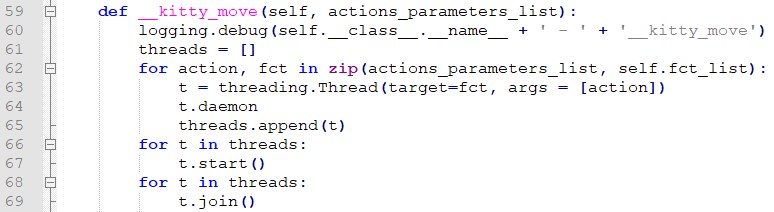
\includegraphics[width=\linewidth]{./images/3_mover}\hfill

    \caption{Mover class}  
    \label{fig:mover}
\end{figure}

The second class, Mover, parallelizes the limbs movement. It has a public method, move, which receives as a parameter a list of movements, loops through each movement and calls the essential method of the class: the private method from figure \ref{fig:mover}. The first parameter of the method, actions\_parameters\_list, is a list of 6 elements corresponding to the 6 elements of the fct\_list. The latter one is a list of functions that controls each limb: \_\_move\_RF (right frontal leg), \_\_move\_RB (right back leg), \_\_move\_LF (left frontal leg), \_\_move\_LB (left back leg), \_\_tail (tail), \_\_head (head). At line 62, each action is correlated with the limb controlling function. While a non-daemonic thread blocks the main thread to exit if they are not dead, daemonic threads do the opposite. This is the reason for line 64. 

The ControlLimb class creates the limb objects: the four legs, one head and one tail. It has a public method to send commands to one limb at a time.   

\subsection*{High-level controller}
Given the low-level controller for moving the entire body of the robot, there is a need for a high-level part to communicate and process the information to and from the user. 

Here is the intelligent agent, giving the package's name "brain". It is responsible for the process of face recognition and emotion detection. There is defined the Python class called Brain (figure \ref{fig:3_brain1}).

\begin{figure}[h]
	\centering
	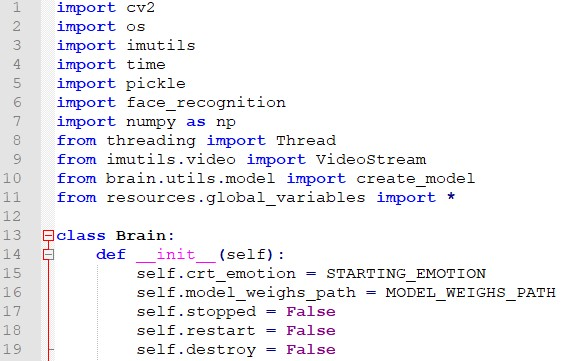
\includegraphics[width=0.7\linewidth]{./images/3_brain1}\hfill	
	\caption{Brain class (1)}  
    \label{fig:3_brain1}
\end{figure}

Lines 1 to 11 handle importing all the necessary packages:
\begin{itemize}

\item cv2 (OpenCV) stands for Open Source Computer Vision Library. It was built to provide a common infrastructure for computer vision applications and to accelerate the use of machine perception in the commercial products\footnote{https://opencv.org/about/}. It has over 2500 optimized algorithms, including a set of both classic and state-of-the-art computer vision and machine learning algorithms. The last version is OpenCV 4.4.

\item os stands for Miscellaneous operating system interfaces\footnote{https://docs.python.org/3/library/os.html};

\item imutils package provide a series of convenience functions to make basic image processing functions\footnote{https://github.com/jrosebr1/imutils};

\item time module offer mostly time-related functions\footnote{https://docs.python.org/3/library/time.html};

\item pickle module implements binary protocols for serializing and de-serializing a Python object structure\footnote{https://docs.python.org/3/library/pickle.html};

\item face\_recognition is package specialized in recognizing and manipulating faces\footnote{https://github.com/ageitgey/face\_recognition};

\item numpy is a math-related package;

\item threading module constructs higher-level threading interfaces on top of the lower level \_thread module\footnote{https://docs.python.org/3/library/threading.html};

\item imutils.video offer the ability to manipulate and use a camera module in an optimized way;

\item the last two imported packages are a part of the application: the first one is CNN's architecture related, while the second one consists of a list of global variables of the application.

\end{itemize}

Lines 14-19 is the constructor of the class. 

\begin{figure}[h]
	\centering
	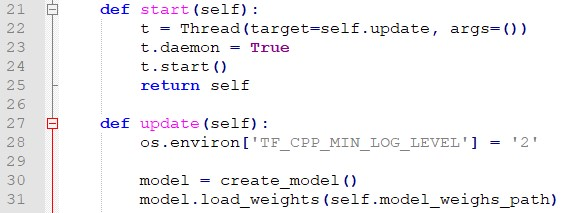
\includegraphics[width=0.7\linewidth]{./images/3_brain2}\hfill	
	\caption{Brain class (2)}  
    \label{fig:3_brain2}
\end{figure}

Lines 21-25 define the start method which invokes  and starts a thread that calls the update method (line 27). By setting the TF\_CPP\_MIN\_LOG\_LEVEL to 2 at line 28, all the info and warning messages from TensorFlow are disabled. The next step is to create a model and its architecture (line 30) and to load the weighs resulted from the last training.

\begin{figure}[h]
	\centering
	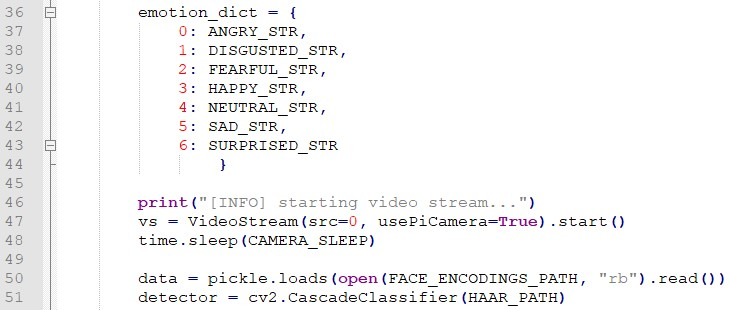
\includegraphics[width=\linewidth]{./images/3_brain3}\hfill	
	\caption{Brain class (3)}  
    \label{fig:3_brain3}
\end{figure}

By convention, all global variables are written in all capital letters with underscore separating words. The dictionary definition at lines 36-44 corellates a key with a string variable signifying an emotion. These will be the strings that will appear on the monitor to communicate the predicted feeling. In case of a non-english user, the string variables' values can be easily translated in other language by changing the global variables file. Lines 47-48 initialize the video stream and allow the camera sensor to warm up. The next 2 lines loads the encoded owner's images and initializes a Haar cascades detector for the face recognition algorithm. 

\begin{figure}[h]
	\centering
	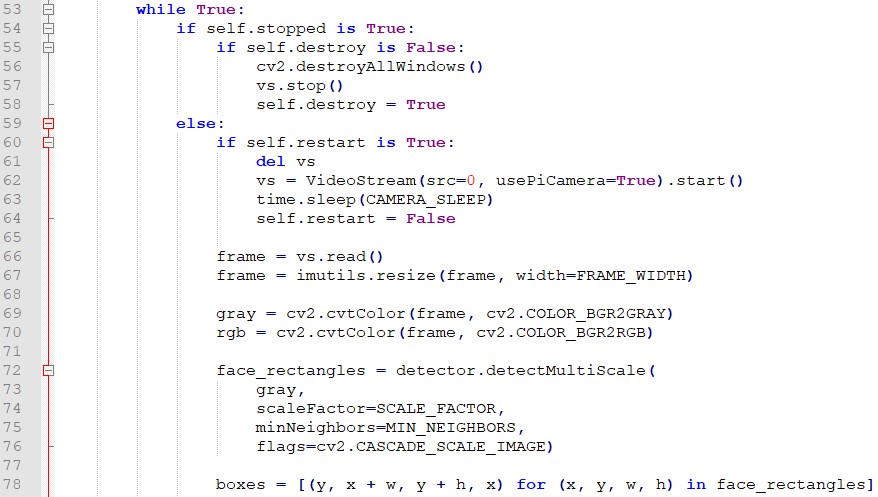
\includegraphics[width=\linewidth]{./images/3_brain4}\hfill	
	\caption{Brain class (4)}  
    \label{fig:3_brain4}
\end{figure}

In figure \ref{fig:3_brain4} an infinite loop starts. Lines 54-64 checks if the camera module is working or not. Then, starting from line 66, a frame is read, resized and converted both to grayscale and RGB. The grayscale resulted image is used for face detection applied by the detector. The detectMultiscale method has 4 parameters: a grayscale image, a parameter which specifies how much the given image is reduced at each image scale, a parameter specifying how many neighbors each candidate rectangle should have to retain it and minimum face size. The result of the face detection is face\_rectangles, a list of bounding boxes corresponding to the located faces in the current frame. Line 78 reorders the bounding box coordinates. OpenCV returns them in the (Ox, Oy, width, height) format and they are rearranged and converted into (top, right, bottom, left).

\begin{figure}[h]
	\centering
	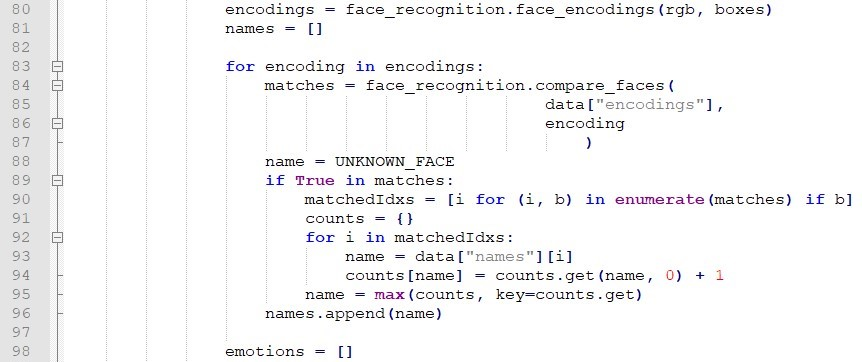
\includegraphics[width=\linewidth]{./images/3_brain5}\hfill	
	\caption{Brain class (5)}  
    \label{fig:3_brain5}
\end{figure}

In figure \ref{fig:3_brain5}, line 80 computes the 128-d encodings for each face, quantifying the face. On lines 83-96, it follows a loop over the facial embeddings in order to compare each detected face from the frame to the already known encodings. Then, a voting system is used to determine whose face it is likely to be, by checking which person in the dataset has the most matches. A list of emotions is created and only the person chosen to be the current owner has the face resized and analyzed by the emotion recognition model (figure \ref{fig:3_brain6}). 

\begin{figure}[h]
	\centering
	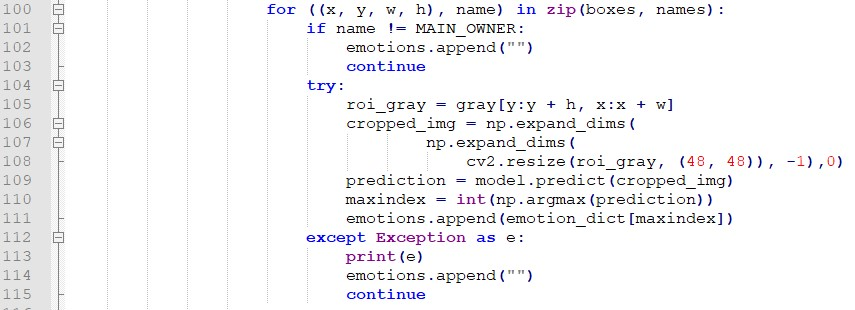
\includegraphics[width=\linewidth]{./images/3_brain6}\hfill	
	\caption{Brain class (6)}  
    \label{fig:3_brain6}
\end{figure}

\begin{figure}[h]
	\centering
	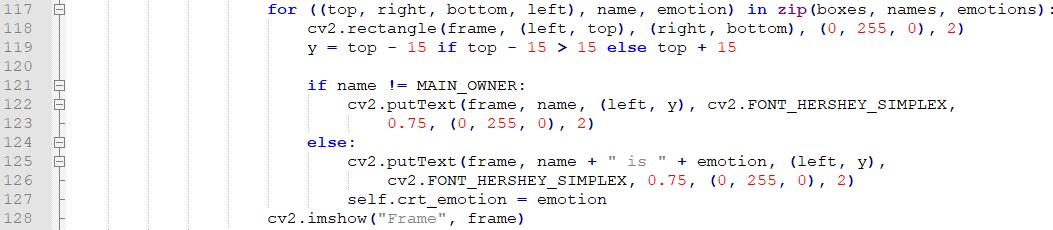
\includegraphics[width=\linewidth]{./images/3_brain7}\hfill	
	\caption{Brain class (7)}  
    \label{fig:3_brain7}
\end{figure}

At the end, in figure \ref{fig:3_brain7} each face has drawn a rectangle surrounding it and only the owner has the emotion predicted. 

\begin{figure}[h]
	\centering
	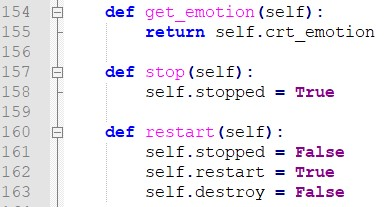
\includegraphics[width=0.5\linewidth]{./images/3_brain8}\hfill	
	\caption{Brain class (8)}  
    \label{fig:3_brain8}
\end{figure}

The last part of this class is represented by 3 short methods (figure \ref{fig:3_brain8}): a getter for the predicted emotion in the current frame, a method to indicate that the thread should be stopped and a method to restart the camera and the prediction algorithm.

================ training

\subsection*{UML diagram}

================== to do

\section{User manual}
\label{chapter:manual}
===================== to do

\section{Experimental results}
\label{chapter:results}

====================== to do

\subsection{Dataset}
\label{subsection:dataset}


\subsection{Configurations}
\label{chapter:configurations}
- dropout pentru reducerea overfitting-ului

- modificarea lr

- a adamului (optimizarii)

- pentru o discutie de final: https://www.kaggle.com/ashishpatel26/tutorial-facial-expression-classification-keras

- pentru o conf matrix: https://github.com/gitshanks/fer2013/blob/master/confmatrix.py

\subsection{Performances}
\label{chapter:performances}
The CNN's architecture was a true challenge given the limitations of the board which could not bear a very deep network. However, according to \cite{fer-cnn}, a 5 layered network would be able to learn discriminative high-level features. For a higher performance, the models were trained with different parameters adjustments. 

In figure \ref{fig:result1}, with a learning rate of 0.001, a decay of $10^{-6}$ and 120 epochs, the best accuracy was 63,14\%. It can be observed that after 20 epochs the model reaches its maximum performance. After this, the accuracy stagnates and the loss easily goes up. Increasing the learning rate at the value 0.01, the results dramatically changed: after the first epoch, the model stagnates at an accuracy of 24,75\% and the training accuracy did not progress more than 25,15\% even after 50 epochs. The reason might be getting stuck in a local minimum because of an improper learning rate. 

\begin{figure}[h]
	\centering
	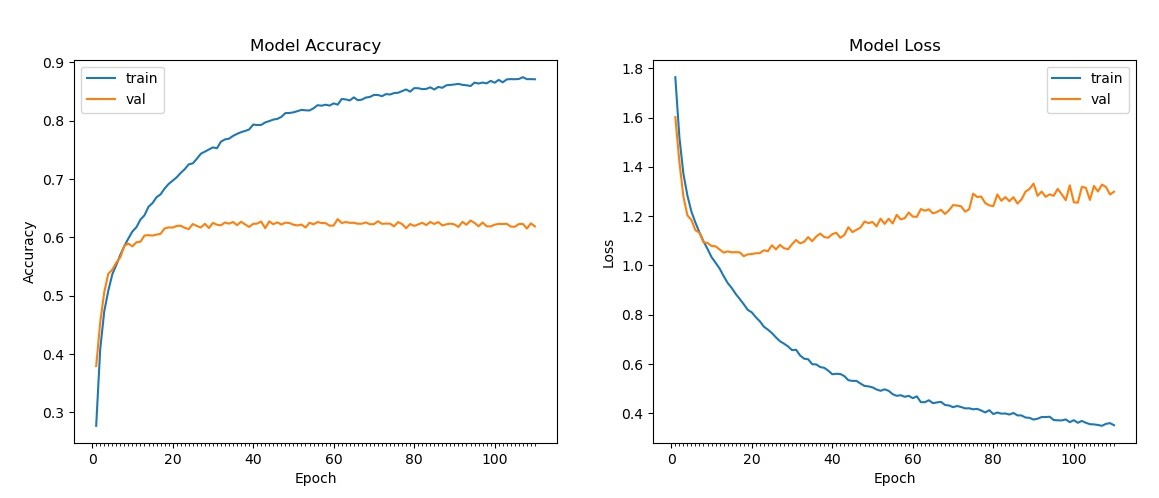
\includegraphics[width=\linewidth]{./images/3_results1}\hfill	
	\caption{Performances: accuracy and loss}  
    \label{fig:result1}
\end{figure}

In figure \ref{fig:result2}, the learning rate was changed to 0.0001. The results were not better. The maximum accuracy was 62,36\% and the values started to stagnate around the 50th epoch. Even after 140 epochs, the accuracy did not improve.

\begin{figure}[h]
	\centering
	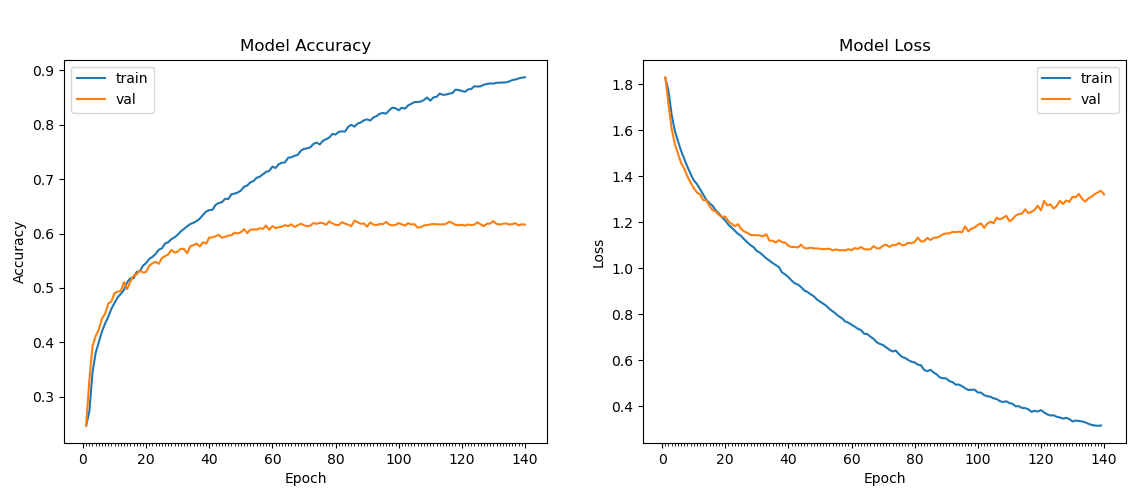
\includegraphics[width=\linewidth]{./images/3_results2}\hfill	
	\caption{Performances: accuracy and loss}  
    \label{fig:result2}
\end{figure}

After supplying the original dataset with the CK+ dataset and a set of personal images (see \ref{subsection:dataset}), the best model was trained. After reaching its maximum performance, the best accuracy was 62,12\%. Although the training accuracy improved faster, per total the model was weaker. 

%======== CONCLUSIONS ========
\chapter*{Conclusions and Future work}
\addcontentsline{toc}{chapter}{CONCLUSIONS}
In this work a social robot called Emotion Cat was designed, built and developed in order to recognize a face using the Viola-Jones algorithm, predict the emotions of its owner using deep learning through a convolutional neural network and react at the resulting emotion. The accurate analysis and interpretation of the human facial expressions is essential for social robots in order to fulfill their purpose, being it medical or for entertainment. Even though, reading a facial expression might happen naturally for a human, for machines it still represents a great challenge. Using hobbyists electronic parts increased the risks and limitations and lead to several crucial tradeoffs, such as the limited number of layers of CNN in order to raise the speed, but decrease the accuracy of the algorithm. 

For future work, there are several improvements that would bring this project closer to realistic standards as a social robot used by people suffering from ASD. The emotion recognition agent could reach a better accuracy if it would analyze the voice tone and the body language of the user. Another improvement would be the integration of an algorithm able to move and calibrate the camera so that the user's face to be centered and easier to read. Better servomotors, with higher torque would help getting over the motion control problems and limitations of the robot. Several sensors, such as ultrasonic sensor for measuring distances or a gyroscope for balance calibrations, would increase the robot's credibility and it would seem more real and practical. And finally, an incorporated battery would confer full autonomy and offer a wider range of expansions of the robot. 

%======== REFERENCES ========
\begin{thebibliography}{9}
\addcontentsline{toc}{chapter}{BIBLIOGRAPHY} 

\bibitem{consumer-robot}
Bertalan Mesk\'o:
\textit{The Top 12 Social Companion Robots},
\texttt{https://medicalfuturist.com/the-top-12-social-companion-robots}

\bibitem{giraff}
Casiddu, Niccolo \& Cesta, Amedeo \& Cortellessa, Gabriella \& Orlandini, Andrea \& Porfirione, Claudia \& Divano, Alessandro \& Micheli, Emanuele \& Zallio, Matteo: 
\textit{Robot Interface Design: The Giraff Telepresence Robot for Social Interaction}, 10.1007/978-3-319-18374-9\_46, (2015),
\texttt{https://www.researchgate.net/publication/300476566\_Robot\_
Interface\_Design\_The\_Giraff\_Telepresence\_Robot\_for\_Social\_Interaction}

\bibitem{bishop}
Christopher M. Bishop:
\textit{Pattern Recognition and Machine Learning}, 
Springer,
2006.

\bibitem{basic-emotions}
Ekman, P.: 
\textit{Basic Emotions}, Handbook of Cognition and Emotion, pp. 45-60, 1999.

\bibitem{mit}
G. Bledt, M. J. Powell, B. Katz, J. Di Carlo, P. M. Wensing and S. Kim:
\textit{MIT Cheetah 3: Design and Control of a Robust, Dynamic Quadruped Robot}, 
2018 IEEE/RSJ International Conference on Intelligent Robots and Systems (IROS), Madrid, 2018, pp. 2245-2252, doi: 10.1109/IROS.2018.8593885.

\bibitem{android-social-skills}
G. Pioggia, R. Igliozzi, M. Ferro, A. Ahluwalia, F. Mura-tori, and D. De Rossi:
\textit{An android for enhancing social skills and emotion recognition in people with autism},
Neural Systems and Rehabilitation Engineering, IEEE Transactions on,13(4):507-515, 2005

\bibitem{sophia}
Hanson Robotics:
\textit{Sophia},
\texttt{https://www.hansonrobotics.com/sophia}

\bibitem{paro}
Hung, Lillian:
\textit{The robotic seal is more than just a companion to patients in hospital wards}, \texttt{https://www.researchgate.net/publication/338852481\_The\_robotic\_seal\_is\_more\_than\_just\_a\_companion\_to\_patients\_in\_hospital\_wards}

\bibitem{deep-learning}
Ian Goodfellow, Yoshua Bengio, Aaron Courville:
\textit{Deep Learning},
MIT Press,
2016,
\\\texttt{www.deeplearningbook.org}

\bibitem{exploration-robot}
Jessica Stoller-Conrad:
\textit{Why do we send robots to space?}, 
\texttt{https://spaceplace.nasa.gov/space-robots/en}

\bibitem{automatic-emotion}
M. Leo et al.:
\textit{Automatic Emotion Recognition in Robot-Children Interaction for ASD Treatment},
2015 IEEE International Conference on Computer Vision Workshop (ICCVW), Santiago, 2015, pp. 537-545, doi: 10.1109/ICCVW.2015.76.

\bibitem{the-cognitive-structure-of-emotions}
Ortony, A., Clore, G., Collins, A.: 
\textit{The Cognitive Structure of Emotions}, Cambridge University Press, Cambridge (1988).

\bibitem{automatic-analysis-of-facial-expressions}
Pantic, M., Rothkrantz, L.J.M.: 
\textit{Automatic analysis of facial expressions: The state of the art}, 
Pattern Anal. Mach. Intell. IEEE Trans.22(12), (2000), 1424-1445.

\bibitem{ik}
Peter Corke:
\textit{Inverse Kinematics for a 2-Joint Robot Arm Using Geometry},
\texttt{https://robotacademy.net.au/lesson/inverse-kinematics-for-a-2-joint-robot-arm-using-geometry}

\bibitem{aerospace-robot}
Piper Thomson:
\textit{6 Types of Robots Shaping Our World},
\texttt{https://learn.g2.com/types-of-robots}

\bibitem{ck}
P. Lucey, J. Cohn, T. Kanade, J. Saragih, Z. Ambadar, and I. Matthews:
\textit{The extended cohn-kanade dataset (ck+): Acomplete dataset for action unit and emotion-specified expression. In Computer Vision and Pattern Recognition Work-shops (CVPRW)}, pages 94-101, June 2010.

\bibitem{the-nature-of-emotions}
Plutchik, R.: 
\textit{The nature of emotions}, 
Am. Sci.89(4), 344-350 (2001).

\bibitem{fer-cnn}
Pramerdorfer, Christopher \& Kampel, Martin:
\textit{Facial Expression Recognition using Convolutional Neural Networks: State of the Art}, 2016, 1612.02903, arXiv, cs.CV. 

\bibitem{reinforcement-learning-introduction} Richard S. Sutton, Andrew G. Barto:
\textit{Reinforcement Learning - An Introduction},
MIT Press,
Cambridge, MA,
1998.

\bibitem{nybble}
Rongzhong Li,
\textit{Nybble - World's Cutest Open Source Robotic Kitten},
\texttt{https://www.indiegogo.com/projects/nybble-world-s-cutest-open-source-robotic-kitten}

\bibitem{how-children-with-asd-behave}
S. M. Anzalone, E. Tilmont, S. Boucenna, J. Xavier, A.-L.Jouen, N. Bodeau, K. Maharatna, M. Chetouani, and D. Co-hen:
\textit{How children with autism spectrum disorder behave andexplore the 4-dimensional (spatial 3d + time) environmentduring a joint attention induction task with a robot},
Research in Autism Spectrum Disorders, 8(7):814 - 826, 2014.

\bibitem{industrial-robot}
Technavio:
\textit{6 Major Types of Industrial Robots Used in the Global Manufacturing 2018}, 
\\\texttt{https://blog.technavio.com/blog/major-types-of-industrial-robots}

\bibitem{mitchell} 
Tom M. Mitchell: 
\textit{Machine Learning},
McGraw-Hill Science/Engineering/Math,
1997.

\bibitem{nao-emotion}
Tutsoy, Onder \& Gongor, Fatma \& Barkana, Duygun \& Kose, Hatice:
\textit{AN EMOTION ANALYSIS ALGORITHM AND IMPLEMENTATION TO NAO HUMANOID ROBOT}, 
The Eurasia Proceedings of Science, Technology, Engineering \& Mathematics (EPSTEM). 1. 316-330, 2017. 

\bibitem{microrobots}
Umai, Devasena \& Parthiban, Brindha \& Thiruchelvi, R.:
\textit{A review on dna nanobots - A new technique for cancer treatment},
Asian Journal of Pharmaceutical and Clinical Research. 11. 61. 10.22159/ajpcr.2018.v11i6.25015. 

\bibitem{medical-robot}
Zachary Tomlinson:
\textit{15 Medical Robots That Are Changing the World},
\texttt{https://interestingengineering.com/15-medical-robots-that-are-changing-the-world}

\end{thebibliography}

\end{document}